\documentclass[11pt,letterpaper]{article}
\usepackage[T1]{fontenc}
\usepackage[utf8]{inputenc}
\usepackage{lmodern,microtype}
\usepackage{amsmath,amssymb,amsthm,mathtools}
\usepackage[margin=0.86in,headheight=15pt]{geometry}
\usepackage{xcolor,booktabs,tabularx,array,enumitem,fancyhdr,hyperref,titlesec,needspace}
\usepackage{tikz}
\usetikzlibrary{arrows.meta,positioning,calc,fit,shapes.geometric}
\usepackage[most]{tcolorbox}
\definecolor{Ink}{HTML}{183047}
\definecolor{Scout}{HTML}{4664A2}
\definecolor{Probe}{HTML}{117A74}
\definecolor{Gold}{HTML}{A87A20}
\definecolor{Pale}{HTML}{F3F7F9}
\definecolor{Rule}{HTML}{D6E1E7}
\hypersetup{colorlinks=true,linkcolor=Scout,urlcolor=Scout,citecolor=Scout,
 pdftitle={Two Armies of One: Certified Scout--Probe Rendezvous, ATLAS Repaired 0.3},
 pdfauthor={<Brian Tenneson>; mathematical development with ChatGPT}}
\titleformat{\section}{\large\bfseries\color{Ink}}{\thesection}{0.7em}{}
\titleformat{\subsection}{\normalsize\bfseries\color{Ink}}{\thesubsection}{0.6em}{}
\setlength{\parindent}{0pt}\setlength{\parskip}{3.4pt}
\setlist{leftmargin=*,itemsep=2pt,topsep=3pt,parsep=0pt}
\pagestyle{fancy}\fancyhf{}
\fancyhead[L]{\footnotesize\sffamily\color{Ink}TWO ARMIES OF ONE}
\fancyhead[R]{\footnotesize\sffamily\color{Probe}ATLAS-REPAIRED 0.3}
\fancyfoot[L]{\scriptsize\color{Ink}Preliminary --- paper-level reasoning, not machine-checked}
\fancyfoot[R]{\scriptsize\color{Ink}\thepage}
\renewcommand{\headrulewidth}{0.35pt}
\newtheorem{theorem}{Theorem}[section]
\newtheorem{proposition}[theorem]{Proposition}
\newtheorem{corollary}[theorem]{Corollary}
\theoremstyle{definition}
\newtheorem{definition}[theorem]{Definition}
\newtheorem{example}[theorem]{Example}
\newtheorem{remark}[theorem]{Remark}
\newtcolorbox{keybox}{enhanced,breakable,colback=Pale,colframe=Rule,boxrule=.7pt,arc=2mm,left=10pt,right=10pt,top=7pt,bottom=7pt}
\newcommand{\C}{\mathcal C}
\newcommand{\vdC}{\vdash_{\mathcal C}}
\newcommand{\nvdC}{\nvdash_{\mathcal C}}
\newcommand{\Adm}{\mathsf{Adm}}
\newcommand{\Mid}{\mathsf{Mid}}
\newcommand{\Used}{\mathsf{Used}}
\newcommand{\Ready}{\mathsf{Ready}}
\newcommand{\PROVED}{\mathsf{PROVED}}
\newcommand{\UNKNOWN}{\mathsf{UNKNOWN}}
\begin{document}
\thispagestyle{plain}
\vspace*{.18in}
{\small\sffamily\bfseries\color{Probe} MATHEMATICAL RESEARCH NOTE \hfill REPAIRED VERSION 0.3\; |\; 26 OCTOBER 2026}\par
\vspace{.30in}
{\color{Ink}\bfseries\fontsize{25}{29}\selectfont Two Armies of One}\par
\vspace{.11in}
{\color{Ink}\fontsize{16}{21}\selectfont Certified Scout--Probe Rendezvous in Proof Search}\par
\vspace{.12in}
{\color{Scout}\large Graft-closed verification, compatible search,\par and the first-settlement barrier}\par
\vspace{.26in}
{\color{Ink}\small Research idea: \textbf{\texttt{\textless{}Brian Tenneson\textgreater{}}}\\ Mathematical exposition and ATLAS-style repair: \textbf{ChatGPT (OpenAI)}}\par
\vspace{.15in}
{\fcolorbox{Gold}{white}{\footnotesize\sffamily\bfseries PRELIMINARY --- REPAIRED, NOT FORMALLY CERTIFIED}}\par
\vspace{.27in}
\begin{keybox}
\textbf{Abstract.} Exactly two search agents are considered: a backward Scout seeking a
checked conditional continuation to a target $T$, and a forward Probe deriving
verified consequences of a frozen hypothesis bank $H$. An accepted Probe proof
$H\vdC L$ can close a compatible Scout proof $H,L\vdC T$; that composition
is sound. For a \emph{fixed} Scout certificate, eventual rendezvous is equivalent
to the Probe eventually recording a \emph{compatible} proof of $L$; under
proof-independent compatibility and fair formula-complete search this
reduces to $H\vdC L$. For a \emph{route-changing}
Scout, fair two-sided enumeration finds a rendezvous whenever a finite,
checker-compatible \emph{admissible triple of certificates} exists. The
structural-midpoint test is decidable on the supplied finite certificates,
not asserted to be decidable for a bare formula. A target-free proper proof cut
(without any claim of semantic necessity) is distinguished from a chronological meeting before direct settlement, which
is \emph{not} guaranteed. The readiness frontier uses actual open proof leaves.
The verifier is now required to accept all locally valid certificates
in the declared MP proof grammar, including legal grafts and opened
subproofs. No speedup, time bound, implementation, proof-assistant
certification, or outside refereeing is claimed.
\end{keybox}
\vspace{.11in}
\begin{center}
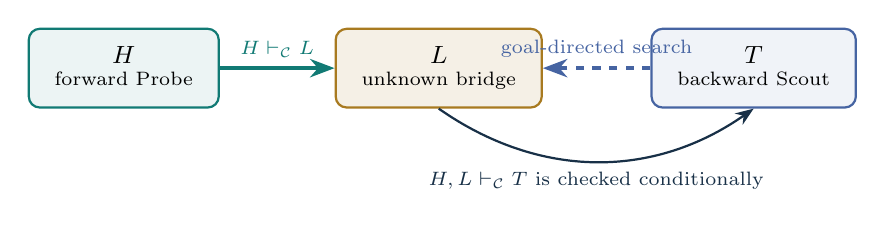
\begin{tikzpicture}[>=Stealth, thick, every node/.style={font=\small}]
\node[draw=Probe,fill=Probe!8,rounded corners=4pt,minimum width=2.35cm,minimum height=1.0cm] (h) at (-4.0,0) {\begin{tabular}{c}$H$\\[-3pt]\scriptsize forward Probe\end{tabular}};
\node[draw=Gold,fill=Gold!11,rounded corners=4pt,minimum width=2.15cm,minimum height=1.0cm] (l) at (0,0) {\begin{tabular}{c}$L$\\[-3pt]\scriptsize unknown bridge\end{tabular}};
\node[draw=Scout,fill=Scout!8,rounded corners=4pt,minimum width=2.35cm,minimum height=1.0cm] (t) at (4.0,0) {\begin{tabular}{c}$T$\\[-3pt]\scriptsize backward Scout\end{tabular}};
\draw[->,Probe,line width=1.3pt] (h)--node[above,font=\scriptsize]{$H\vdC L$}(l);
\draw[->,Scout,dashed,line width=1.3pt] (t)--node[above,font=\scriptsize]{goal-directed search}(l);
\draw[->,Ink] (l.south) to[out=-35,in=-145] node[below,font=\scriptsize]{$H,L\vdC T$ is checked conditionally} (t.south);
\end{tikzpicture}
\end{center}
\begin{center}\footnotesize\itshape The dashed arrow is search direction, not a reverse logical inference.\end{center}
\clearpage

\section{Question, architecture, and claim levels}
There are \emph{two armies of one}: one Scout and one Probe. Their meeting point
need not be specified in advance. Both may search indefinitely, and matching
and checking are operations of their common protocol, not additional search agents.
The word \emph{certificate} has a strict meaning: a finite proof object accepted
by the stated verifier. An unverified candidate is only a proposal.

Three claims must remain distinct:
\begin{enumerate}[label=\textbf{\arabic*.}]
\item \textbf{Composition soundness:} two compatible certificates certify $T$.
\item \textbf{Conditional eventual discovery:} a finite eligible matching pair is
 eventually detected by a search that is fair, persistent, and allowed to continue.
\item \textbf{A useful early meeting:} an eligible lemma is found before either agent
 independently proves $T$, perhaps at less total cost than a matched comparator.
\end{enumerate}
Only the first two are established under explicit assumptions. The third
requires a separate result or experiment.

\section{Formal setting and certificate discipline}
Fix a countable effectively encoded propositional or first-order presentation
$\C$ whose \emph{only proper inference rule is modus ponens} (MP).
Assume decidable axiom-instance membership and decidable membership in the
frozen authorized hypothesis bank $H$.

\begin{definition}[Full local MP certificate grammar]\label{def:grammar}
For a finite set $O$ of \emph{designated open occurrences}, a certificate is a
finite acyclic proof DAG with a distinguished conclusion node. Every leaf is
an accepted axiom instance, a member of $H$, or one of the explicitly open
formula occurrences from $O$. Each internal node is a legal MP inference,
whose \emph{ordered} input formulas are $A$ and $A\to B$ and whose output
formula is $B$. A node may be shared by several downstream uses. Imports
must be expanded or carry recursively checkable, scope-correct receipts.
\emph{Correctness} means satisfaction of all these local conditions and
all stipulated formula/type/substitution rules of the declared presentation.
The verifier $V$ \emph{decides this correctness predicate in both directions}:
$V(\sigma)=\mathsf{accept}$ if and only if $\sigma$ is a correct finite
certificate in this declared grammar and context. Thus it is not allowed
an additional global length or resource cap while being used for these theorems.
\end{definition}

The relevant closure conditions follow from this explicit grammar and are
also required of implementations with opaque receipt formats:
\begin{enumerate}[label=(\roman*)]
\item \emph{Heredity:} extracting the complete ancestor sub-DAG at any node,
with its inherited $H$ and axiom leaves, yields a checkable proof of that node;
\item \emph{Opening:} replacing one internal proof occurrence by an open leaf
of the same formula in the remaining trimmed proof yields an accepted
conditional certificate, when its other dependencies are retained;
\item \emph{Grafting:} replacing a designated open leaf by a finite checked
proof of the same formula from $H$ yields a checked finite certificate
whenever the contexts, scopes, substitutions and imported receipts are
compatible. The resulting proof may be arbitrarily longer than either input.
\end{enumerate}
These are operations on proof occurrences, not reverse inference rules.
Trimming deletes nodes outside the ancestry of the distinguished conclusion;
for target-free tests, imports are fully expanded or their complete provenance
is inspectable. A ledger cannot silently rewrite $H$, add axioms, or exchange
calculus or verifier. Fair enumeration of finite strings is possible; this
in no way decides theoremhood.

\begin{definition}[Probe and Scout certificates]
A Probe certificate $\pi_L$ is a finite checked proof $H\vdC L$ with no
unresolved assumptions. A Scout certificate $\rho_L$ is a finite checked
\emph{conditional} proof $H\cup\{L\}\vdC T$ whose trimmed conclusion ancestry
contains a distinguished \emph{open leaf} labeled $L$. The Scout has not thereby
proved $H\vdC T$. These are proof occurrences, not merely matching formula names.
\end{definition}

\begin{definition}[Proof-specific compatibility and certified rendezvous]
Let $\mathsf{Comp}(\pi,\rho)$ be the terminating predicate that checks that
$\pi$ proves the formula at every designated open occurrence of $\rho$ to
be grafted, that the entire finite graft respects the frozen context, all
proof-occurrence scopes and imports, and that the resulting certificate is
correct under $V$. A rendezvous at $L$ is recorded only after checking
$V(\pi_L)=V(\rho_L)=\mathsf{accept}$,
$\mathsf{Comp}(\pi_L,\rho_L)=\mathsf{true}$, and
$V(\rho_L[\pi_L/L])=\mathsf{accept}$.
The notation denotes grafting into all designated open $L$ leaves.
For the full grammar of Definition~\ref{def:grammar}, two certificates
with the same frozen $H$ and permitted imports are compatible by
construction. Under extra provenance restrictions, compatibility may depend
on the \emph{particular Probe certificate}, not merely its conclusion $L$.
A planned reverse edge is \emph{not} an inference of a premise from a
conclusion.
\end{definition}

\begin{remark}[The original calculus remains a dependency]
An MP-only presentation $F^\star$ may be instantiated as $\C$. The claim
that a proof in $F^\star$ can be decoded into an original first-order
presentation $F$ belongs to a \emph{separate} translation theorem and audit.
No result in this note independently proves that translation correct.
\end{remark}

\section{Soundness of certificate composition}
\begin{theorem}[Certified composition under graft closure]\label{th:compose}
Let $\pi_L$ be a $V$-accepted $H\vdC L$ proof and let $\rho_L$ be a
$V$-accepted conditional $H,L\vdC T$ proof with distinguished open
$L$ occurrences. Suppose their complete contexts and receipt dependencies
are compatible as in Definition~\ref{def:grammar}. Then legal grafting
constructs a finite $V$-accepted proof $H\vdC T$.
\end{theorem}
\begin{proof}
Trim $\rho_L$ to the ancestry of $T$ and replace each open $L$ occurrence
by a fresh copy of the closed $H$-proof $\pi_L$ (or an equivalent
verified import). The insertion cannot create a directed cycle: its
fresh finite sub-DAGs do not depend on the Scout's open leaves. All
remaining leaves belong to $H$ or the axiom stock. All original MP
ports retain the same premise formulas and conclusion; inserted MP nodes
were checked already. The new finite DAG therefore satisfies the grammar
of Definition~\ref{def:grammar}. Since $V$ accepts every correct certificate
in that grammar, the new proof is accepted and concludes $T$ from $H$.
\end{proof}

\begin{remark}[Soundness alone is insufficient: an explicit failure]\label{rem:cap}
In the propositional MP system with $H=\{p,p\to \ell,\ell\to t\}$,
let $V_1$ check local correctness but reject any proof using more than
one MP inference. This is a \emph{sound terminating} certificate checker.
It accepts the one-step $H\vdash \ell$ certificate and the one-step
$H,\ell\vdash t$ conditional certificate, but rejects their two-step
composite. Theorem~\ref{th:compose} therefore needs full validity
recognition or explicit graft closure; mere soundness of $V_1$ does not
suffice. The theorem makes neither an efficiency nor a small-proof claim.
\end{remark}

\begin{corollary}[Conditional return translation]
If there additionally exists a separately validated total decoder
$D$ mapping checked $\C$-proofs of $H\vdC T$ into checked proofs of
$H\vdash_F T$, then applying $D$ to the composite proof yields such an
$F$-proof, provided the final $F$ checker accepts it.
\end{corollary}

\begin{remark}[Why assumption scope is not cosmetic]
In a calculus whose rules include assumption-sensitive generalization,
blind proof insertion can invalidate a rule because its premise acquires
new open support. The theorem intentionally concerns the specified MP-only
certificate format; it does not license unsupported proof splicing in an
arbitrary calculus.
\end{remark}

\section{One fixed Scout route: the exact eventuality theorem}
\begin{definition}[Probe enumeration and fair matching]
Let $E_P(L)$ be the set of accepted $H$-proof certificates concluding
$L$ \emph{actually recorded} by the Probe in a continuing run. A
\emph{formula-complete} Probe eventually records at least one such proof
for every provable $L$. A \emph{certificate-complete} Probe eventually
records every finite $V$-accepted $H$-proof object (up to the declared
finite encoding). In both cases records persist and the matcher fairly
examines every recorded pair with the fixed Scout certificate. Continued
operation has no finite budget or early-stop rule.
\end{definition}

\begin{theorem}[Fixed-Scout rendezvous: exact compatibility criterion]
\label{th:fixed}
Fix a checked Scout certificate $\rho_L:H,L\vdC T$ with a used
open occurrence $L$. With persistent accepted certificates, fair matching,
and continued operation, the protocol eventually rendezvous at $L$ if
and only if
\[
   \exists\pi\in E_P(L)\quad\mathsf{Comp}(\pi,\rho_L)=\mathsf{true}.
\]
If the Probe is certificate-complete this is equivalent to the existence
of \emph{some} compatible checked $H$-proof of $L$. If the Probe is only
formula-complete, the simpler equivalence
\[
   \text{eventual meeting at $L$}\quad\Longleftrightarrow\quad H\vdC L
\]
holds when every accepted $H$-proof of $L$ is compatible with the fixed
Scout certificate, as in the full, shared-context grammar above.
\end{theorem}
\begin{proof}
For the first equivalence, an eventual rendezvous has an actual
recorded, compatible Probe witness. Conversely, any witness in $E_P(L)$
is recorded at some finite stage. Persistence and fair matching ensure
that it is eventually tested; compatibility and
Theorem~\ref{th:compose} certify the splice. Under certificate
completeness, all finite proofs are eventually in $E_P(L)$.
For the last assertion, formula completeness supplies an accepted
$H$-proof whenever $H\vdC L$, and uniform compatibility makes
that proof eligible; the converse follows from soundness. None of these
equivalences implies a finite uniform bound on the meeting stage.
\end{proof}

\begin{remark}[Why the proof-specific qualification is essential]
If a receipt rule accepts one derivation of $L$ but rejects another,
a formula-complete Probe might record only the rejected one. Then
$H\vdC L$ does \emph{not} imply rendezvous for that particular schedule.
The existential proof-witness formulation handles these cases without
assuming compatibility from a matching formula label alone.
\end{remark}

\begin{example}[A stranded Scout despite a provable target]\label{ex:stranded}
In the classical propositional fragment take
\[
 H=\{p,p\to t,q\to t\},\qquad T=t,\qquad L=q.
\]
The Probe can establish $t$ using $p,p\to t$. The Scout's conditional
route from $q$ to $t$ is checked using $q\to t$, but $H\nvdash q$:
the valuation $p=t=\mathrm{true}$ and $q=\mathrm{false}$ satisfies $H$
and refutes $q$. Thus that fixed Scout cannot meet the Probe at $q$.
The provability of $T$ alone is insufficient for an arbitrary fixed $L$.
\end{example}

\section{A Scout that changes routes: conditional completeness}
\begin{definition}[Fair two-sided proof search]
The Scout fairly enumerates all finite, accepted conditional objects
$(L,\rho)$ using an open $L$ leaf to derive $T$ from $H,L$. The Probe
fairly enumerates all finite checked proofs $\pi$ from $H$, or at least
one accepted proof for every derivable conclusion when no certificate-sensitive
filter is used. For a predicate depending on the \emph{particular Probe proof},
full finite-certificate coverage is required. Certificates persist, and
a dovetailed matcher fairly tests jointly available triples $(L,\pi,\rho)$.
Neither search is allowed to terminate upon an unrelated proof if an
eventual detection result for a specified witness is being asserted.
\end{definition}

\begin{definition}[Computable witness admissibility]
An admissibility rule $\Adm(L,\pi,\rho)$ is a total terminating algorithm
on an explicitly supplied finite triple. It may test formula syntax,
contexts, scope closure, dependency graphs, target occurrences, and
provenance receipts. It is \emph{not} a decision procedure for the
unbounded claim ``there exists some admissible proof triple for $L$.''
\end{definition}

\begin{theorem}[Witness-filtered eventual rendezvous]\label{th:witness}
Assume the setting above with fair two-sided \emph{full-certificate}
enumeration, persistent records, fair matching, and continued unbounded
execution. If there exists a compatible finite triple $(L,\pi_L,\rho_L)$
such that
\[
 \pi_L:H\vdC L,\qquad \rho_L:H,L\vdC T,
 \qquad \Adm(L,\pi_L,\rho_L)=\mathrm{true},
\]
then the two-agent protocol eventually detects and certifies an
$\Adm$-admissible rendezvous (possibly via a different qualifying triple).
\end{theorem}
\begin{proof}
The witness consists of finitely encoded proof objects. Fair enumeration
eventually places its Scout and Probe records in persistent storage.
Fair triple matching eventually tests that pair. Because $\Adm$ is
terminating and accepts the given compatible triple, and splicing is
checked, Theorem~\ref{th:compose} establishes the rendezvous. The
argument guarantees no order relative to a separate direct proof of $T$.
\end{proof}

\subsection{The deliberately weak guarantee at $L=T$}
If $H\vdC T$ and the policy permits $L=T$, the Scout has a one-leaf
conditional certificate $H,T\vdC T$ while the Probe eventually discovers
a checked $H\vdC T$ proof. This is a valid but \emph{degenerate} meeting:
Probe completion of $T$ already settles the target. It is incorrect to
promote this statement into a guarantee of a useful internal bridge.
Conversely, when $L=T$ is excluded, target provability by itself supplies
\emph{no} witness to Theorem~\ref{th:witness}.

\section{What can ``somewhere in the middle'' mean?}
\begin{definition}[Target-free structural witness cut]\label{def:mid}
For fully expanded, compatible finite certificates define
$\Mid(L,\pi,\rho)$ to hold when all the following finite checks pass:
\begin{enumerate}[label=(\roman*)]
\item $L\neq T$ and $L\notin H$ as literal formula membership;
\item the trimmed Probe certificate $\pi$ ends at $L$, contains at least
 one proper inference step, and contains \emph{no occurrence of $T$ anywhere
 in its disclosed nodes};
\item the trimmed Scout certificate $\rho$ contains a designated open leaf
 $L$ in the concluding $T$'s ancestry, with a nonempty chain containing
 at least one proper inference step from that leaf to the final $T$;
\item exact contexts, supports, ordered MP ports, imported receipts, and
 the complete splice pass verification.
\end{enumerate}
This is a \emph{certificate-relative target-free cut}---not a declaration
that the meeting is efficient or temporally earlier than direct settlement.
\end{definition}

The predicate $\Mid$ is decidable \emph{given the finite expanded witnesses}.
A program tests syntactic equality, ancestry in finite acyclic graphs,
inference-node counts, and proof checking. This does not assert that
$\{L:\exists\pi,\rho\ \Mid(L,\pi,\rho)\}$ is decidable.

\begin{proposition}[Conditional detection of a target-free cut]\label{prop:mid}
If one compatible triple satisfies $\Mid$, then the continuing, fully
fair two-agent protocol using $\Adm=\Mid$ eventually detects such a
certificate-relative cut and completes a checked proof of $T$.
\end{proposition}
\begin{proof}
The four clauses of Definition~\ref{def:mid} give a total predicate on
the supplied finite triple. Apply Theorem~\ref{th:witness}.
\end{proof}

\begin{proposition}[A certified DAG cut supplies a bridge]\label{prop:cut}
Suppose a finite, verified, trimmed proof DAG of $H\vdC T$ contains an
internal occurrence $v$ labeled $L\notin H\cup\{T\}$. Suppose $v$ has
at least one inference ancestor, lies on a directed path to the final
$T$ through a proper inference step, and its ancestor sub-DAG has no
node labeled $T$. then severing $v$ yields compatible Probe and Scout
certificates satisfying $\Mid$, provided the verifier accepts ancestor
extraction and opening as in Definition~\ref{def:grammar}.
\end{proposition}
\begin{proof}
By heredity, the ancestry at $v$ is an $H$-proof $\pi_L$; expand imports
and keep all premise dependencies. In a copy of the original DAG,
use opening to replace $v$ by a distinguished open $L$ leaf and discard now-unneeded
nodes; this is a checked conditional proof $\rho_L$ of $T$ from $H,L$.
The designated leaf remains on a dependency path to $T$. All four
finite checks in Definition~\ref{def:mid} follow from the hypotheses;
splicing restores a valid proof of $T$.
\end{proof}

\begin{remark}
This proposition does not assert that every provable target has such a
cut. It gives a sufficient structural criterion for the existence of a
witness. It also does not impose a cost advantage on the agents that find it.
\end{remark}

\subsection{Two precise counterexamples to overclaiming}
\begin{example}[A false midpoint: a target-first detour]\label{ex:detour}
Work in a classical propositional MP-only Hilbert presentation with
ordinary tautology axioms, and set
\[
 H=\{p,p\to t\},\quad T=t,\quad U=(q\to q),\quad L=t\land U.
\]
There is a checked Probe derivation of $t$ from $p,p\to t$, followed by
a derivation of $U$ and a derived conjunction-introduction proof of
$L$. A Scout can use the conditional leaf $L$ and the propositional
theorem $(t\land U)\to t$ to derive $t$. Thus $L\notin H$, $L\neq T$,
and the spliced proof has nonzero work on both sides. \emph{Nevertheless
$T$ occurred in the Probe proof before $L$.} The old syntactic and
proper-cut criteria wrongly classified this as an informative middle
meeting. Condition (ii) of $\Mid$ rejects the triple.
\end{example}

\begin{example}[A target-free certificate cut need not be early]\label{ex:notearly}
Let $H=\{p,p\to \ell,\ell\to t\}$ and $T=t$, $L=\ell$.
The one-step MP proof of $\ell$ and conditional MP continuation
from $\ell$ to $t$ satisfy $\Mid$. But a fair search schedule can
complete and record an entirely separate proof of $t$ \emph{before}
its Probe and Scout enumerations jointly expose that cut. Fairness
constrains eventual inclusion, not the relative order of discoveries.
So $\Mid$ is \emph{not} a guarantee of an early runtime rendezvous.
\end{example}

\begin{example}[A target-free cut can be logically inessential]\label{ex:inessential}
Let $H=\{t\}$ and $T=t$. Choose $L=(q\to q)$, which has an MP-based
closed proof using only propositional axiom instances involving $q$.
Take such a proof with at least one MP step as the Probe certificate;
it contains no occurrence of $t$. For the Scout, use the axiom
$t\to(L\to t)$, the hypothesis $t$, and MP to obtain $L\to t$;
then use the open $L$ and MP to obtain $t$. Both selected proof branches
contain proper inference steps, and the triple passes $\Mid$.
Nevertheless $H\vdC T$ has the one-line hypothesis proof, without any
rendezvous. Thus even the repaired structural predicate establishes
only a \emph{target-free certificate cut}, not that $L$ is mathematically
necessary or operationally worthwhile.
\end{example}

\begin{remark}[Why global logical necessity is the wrong requirement]
For any successful rendezvous the composition theorem already gives
$H\vdC T$. It would therefore be self-defeating to define a useful
bridge by requiring $H\nvdC T$ when $L$ is omitted: that condition
cannot coexist with a successful proof of $T$ from $H$. Use a specified
proof DAG, chronology, or a charged comparison to describe usefulness,
never an assertion that $L$ is globally indispensable to consequence.
\end{remark}

\begin{keybox}
\textbf{Chronological first-settlement distinction.} Let $s_L$ be the
actual step when compatible $L$-certificates are first joined, and
$s_T$ the step at which an unassisted branch of the declared run first
produces an accepted $H\vdC T$ proof. A \emph{pre-settlement} meeting
would require $s_L<s_T$, with the event history and cost model fixed
in advance; define $s_T=+\infty$ if that independent branch never
produces such a proof. Theorem~\ref{th:witness} makes no such assertion. Some
runs terminate at $s_T$ before any eligible rendezvous is detected;
those runs do not satisfy the continuing-search premise used for the
eventual-admissible-witness claim.
\end{keybox}

\section{A correctly drawn two-army example}
Let $H=\{P,P\to L,L\to T\}$. The following is a two-MP proof with a
precise meeting occurrence and two proper inference nodes:
\begin{center}
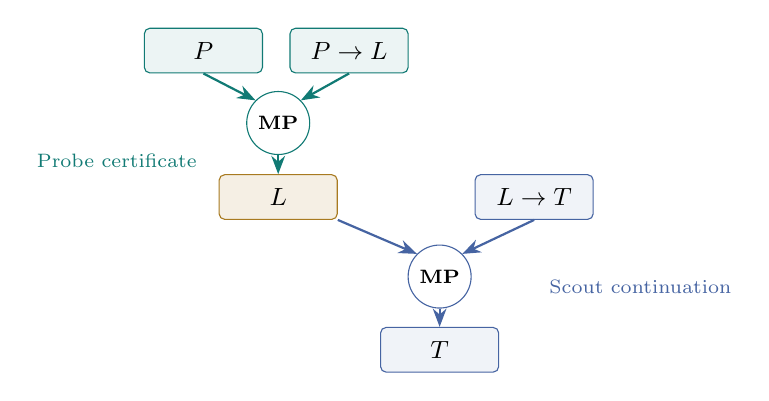
\begin{tikzpicture}[>=Stealth, every node/.style={font=\small},
 pbox/.style={draw,rounded corners=2pt,inner sep=5pt,minimum width=15mm},
 mp/.style={draw,circle,fill=white,minimum size=8mm,inner sep=1pt,font=\scriptsize\bfseries}]
\node[pbox,fill=Probe!8,draw=Probe] (p) at (-3.9,1.8) {$P$};
\node[pbox,fill=Probe!8,draw=Probe] (imp1) at (-2.05,1.8) {$P\to L$};
\node[mp,draw=Probe] (mp1) at (-2.95,.88) {MP};
\node[pbox,fill=Gold!12,draw=Gold] (l) at (-2.95,-.06) {$L$};
\node[pbox,fill=Scout!8,draw=Scout] (imp2) at (0.3,-.06) {$L\to T$};
\node[mp,draw=Scout] (mp2) at (-.9,-1.07) {MP};
\node[pbox,fill=Scout!8,draw=Scout] (t) at (-.9,-2.0) {$T$};
\draw[->,Probe,thick] (p.south) -- (mp1.north west);
\draw[->,Probe,thick] (imp1.south) -- (mp1.north east);
\draw[->,Probe,thick] (mp1.south)--(l.north);
\draw[->,Scout,thick] (l.south east) -- (mp2.north west);
\draw[->,Scout,thick] (imp2.south) -- (mp2.north east);
\draw[->,Scout,thick] (mp2.south)--(t.north);
\node[font=\scriptsize\color{Probe}] at (-5.0,.4) {Probe certificate};
\node[font=\scriptsize\color{Scout}] at (1.65,-1.2) {Scout continuation};
\end{tikzpicture}
\end{center}
The Probe certifies $H\vdC L$. The Scout presents a checked conditional
proof $H,L\vdC T$ using the $L$ leaf and $L\to T$. At rendezvous the
certified $L$ occurrence closes the Scout leaf. The diagram does not
pretend that $L$ follows from $T$.

\section{One Scout with several genuinely open obligations}
A conditional proof of $T$ may require a \emph{finite set} of open leaves,
not just one. No third agent is required: the same Probe can certify
several lemmas over time.

\begin{definition}[Exact obligation support]
For a checked, trimmed conditional certificate $\rho$ whose declared
open labels lie in a finite set $O$, define
\[
 \Used(\rho)=\{L:\text{an open leaf labeled $L$ occurs in the
 ancestry of its designated final $T$}\}.
\]
This is the actual \emph{syntactic} obligation support of that proof
occurrence, not the set of all formulas that were offered to it. The
support may not be semantically minimal across all alternative proofs.
\end{definition}

\begin{proposition}[Exact finite discharge]\label{prop:sets}
If $\rho:H\cup O\vdC T$ is a finite checked conditional proof and
every $L\in\Used(\rho)$ has a compatible checked $H$-proof, then
finite proof splicing yields a checked $H$-proof of $T$.
Under a continuing \emph{certificate-complete} Probe, persistence, and
fair matching, any specified finite set $\Used(\rho)$ for which
there exist \emph{jointly compatible} checked discharge certificates
is eventually completed. A merely formula-complete Probe suffices if
all checked $H$-proofs of these formulas are uniformly graft-compatible.
\end{proposition}
\begin{proof}
Only the open leaves in the trimmed final ancestry matter. Replace
their occurrences by the compatible $H$-proofs, check the finite
composite, and obtain $H\vdC T$. For eventuality, certificate completeness records each member of a
chosen jointly compatible finite family of witnesses; its maximum
arrival stage is finite. Fair matching eventually performs the
finite composite, which $V$ accepts by repeated graft closure.
\end{proof}

For a \emph{fixed finite family} of already checked conditional routes
$\rho_1,\ldots,\rho_m$ over one common verifier/context with compatible
receipts, put $O_i=\Used(\rho_i)$ and let $B$ denote the set of
currently available certified $H$-conclusions. Within this particular
family, and under the compatibility assumption,
\[
 \Ready(B)=\bigvee_{i=1}^m [O_i\subseteq B].
\]
Deleting a set $O_j$ that strictly contains another listed $O_i$
does not change this readiness predicate. Thus the distinct inclusion-minimal
$O_i$ form an antichain \emph{for the selected finite family}. If receipt
compatibility varies between routes, the correct frontier uses
context-qualified proof receipts rather than plain formula-set inclusion.
This is not the same object as a history-unfolded SIC frontier.

\section{A fair protocol and its stopping policy}
\begin{keybox}
\textbf{Schematic two-agent protocol (no experimental execution claimed).}
\begin{enumerate}[label=\textbf{\arabic*.}]
\item Freeze $\C,H,T,V$, the admissibility predicate, receipts, schedule, and charged costs.
\item Dovetail Scout enumeration of finite checked conditional certificates
 (single leaves or declared finite sets). Keep rejected proposals in
 $\mathsf{CAND}$, not in a certified lemma bank.
\item Dovetail Probe enumeration of finite checked $H$-proofs. Append
 checker-accepted certificates to a persistent provisional ledger; do
 not silently mutate the frozen hypothesis bank.
\item Fairly enumerate jointly available certificate pairs/triples;
 check exact contexts and imports, then apply $\Adm$ on the \emph{full witness}.
\item On successful splicing and a final $V$ pass, record a certified
 $H\vdC T$ conclusion. Invoke a return decoder only if that decoder
 has separately passed its audit.
\item If the goal is guaranteed detection of an eligible witness,
 continue searching until it is detected; an earlier, unrelated
 $H$-proof of $T$ must not stop that special search. In a normal
 first-settlement run, report the first verified result and do
 \emph{not} claim the same eventual eligible-witness guarantee.
\item Under a finite budget, if no accepted terminal result is produced,
 report $\UNKNOWN$ rather than treating failure to meet as a refutation.
\end{enumerate}
\end{keybox}

A fair rescue enumeration may coexist with heuristics, but it must not
be starved if its eventuality guarantee is invoked. Each proof check,
proposal, import, match, storage operation, and final verification must
be charged under an explicitly declared machine and budget model.
For example,
\[
 W=W_{\rm Scout}+W_{\rm Probe}+W_{\rm check}+W_{\rm match}
 +W_{\rm store}+W_{\rm compose}+W_{\rm decode}+W_{\rm final}.
\]
The above mathematical assumptions do not provide a general quantitative
upper bound for $W$, nor do they establish a speedup over an equally
resourced prover allowed both forward and backward search.

\section{Status of every research claim}
\small
\begin{tabularx}{\linewidth}{@{}>{\raggedright\arraybackslash}p{0.37\linewidth}X@{}}
\toprule
\textbf{Claim} & \textbf{Correct status}\\\midrule
Sound splicing of compatible MP certificates & Proven for the declared graft-closed grammar and compatible receipts (Theorem~\ref{th:compose}).\\
Fixed-route rendezvous & Exact iff requires a recorded compatible proof; iff $H\vdC L$ also needs uniform compatibility and formula completeness (Theorem~\ref{th:fixed}).\\
Changing-route Scout finds an existing eligible triple & Proven with full-certificate fairness, compatibility, persistence, graft closure, and continuing execution (Theorem~\ref{th:witness}).\\
Guaranteed useful midpoint from $H\vdC T$ alone & \textbf{Not proved; false as a claimed consequence of the assumptions.} Only $L=T$ is universally available if allowed.\\
Certificate-relative target-free proper cut & Decidable for a given finite triple; existence requires an additional witness (Definition~\ref{def:mid}, Proposition~\ref{prop:mid}).\\
Meeting before first direct proof of $T$ & \textbf{Not guaranteed}; depends on actual schedule and run (Example~\ref{ex:notearly}).\\
Semantic necessity of the bridge & \textbf{Not guaranteed}, even for a target-free cut (Example~\ref{ex:inessential}).\\
Strictly lower fully charged cost & Open; no measurements presented.\\
Decoding from $F^\star$ to original calculus $F$ & Dependent on a separate verified decoder and final original checker.\\
Working two-agent prover / formal proof assistant certification & Not supplied or claimed.\\
\bottomrule
\end{tabularx}
\normalsize

\section{Correction history and open problems}
Version 0.3 repairs the fresh 26 October 2026 ATLAS-style audit of
version 0.2, incorporating explicit verifier heredity/opening/graft
closure, proof-specific compatibility quantifiers, and the $s_T=+\infty$
convention. It preserves the previously repaired midpoint and
no-speedup distinctions. The preceding version 0.2
had replaced the misleading formula-only ``middle'' test, rejected a
spurious target-first proper-cut example, and separated structural cuts
from chronological runtime advantage. The precise
correction ledger accompanies this manuscript as a separate file.

The open mathematical questions are whether natural infinite target families
admit useful internal cuts with controllable costs, whether an independently
scheduled Scout and Probe can encounter such cuts before direct settlement,
and whether their charged cost beats a matched, equally capable baseline.
The formal results above \emph{do not} answer those questions affirmatively.

\textbf{Publication designation: PRELIMINARY / ATLAS-REPAIRED v0.3.}
The repaired results have undergone a fresh ATLAS-style paper-level
re-audit; this does not constitute independent third-party refereeing,
proof-assistant formalization, an implemented system, or benchmarking. It is not a certified theorem-bank
receipt and does not authorize a live AMLD experiment.

\begin{thebibliography}{9}\setlength{\itemsep}{1.5pt}
\bibitem{orig} B. Tenneson, \emph{Two Armies of One: Certified Scout--Probe Rendezvous in Proof Search}, v0.1, 26 October 2026.
\bibitem{audit1} \emph{ATLAS Independent Audit: Two Armies of One v0.1}, first paper-level audit, 26 October 2026.
\bibitem{audit2} \emph{ATLAS: Fresh Mathematical Re-Audit of Two Armies of One}, audit 0.2, 26 October 2026.
\bibitem{trading} B. Tenneson, \emph{Trading, Intuition, and Return}, v0.1, preliminary companion note, 26 October 2026.
\bibitem{audit3} \emph{ATLAS: Fresh Independent Audit of Two Armies of One v0.2}, specification audit, 26 October 2026.
\bibitem{openakm} B. Tenneson, \emph{OPEN. AKM}, v0.2, preliminary theoremgraph-reversal companion, October 2026.
\end{thebibliography}
\end{document}
